
A solução envolve quatro componentes essenciais, que interagem para formar a solução definida. Dois destes componentes são a fonte de dados primária, que inicialmente é indicada como o Matrícula Web, e o mecanismo de extração das informações. O terceiro componente é a API de consulta de informações, que enolve a formatação semântica e inferência sobre das informações utilizadas. Por fim, o último componente constitui a camada de aplicação, envolvendo o sistema de recomendações e a representação das informações através do Portal FGA.

\begin{figure}[H]
	\centering
	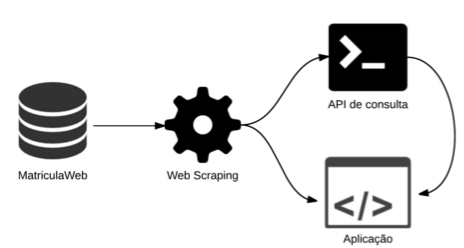
\includegraphics[width=0.7\textwidth]{imagens/estrutura}
	\caption{Estrutura da Solução}
	\label{img:estrutura}
\end{figure}

\subsubsection{Fonte de Dados e Extração} % (fold)
\label{ssub:fonte_de_dados_e_extra_o}

	Como dito, espera-se utilizar o \href{http://matriculaweb.unb.br}{\textbf{Matrícula Web}} como fonte de dados primária, provendo todos os dados referentes aos fluxos e ofertas de disciplinas. No entanto, não existe uma API disponíel para consulta, o que aumenta a complexidade da atividade de extração de informações.

	Por este motivo, parte de um dos componentes fundamentais para a aplicação é um serviço de \textit{Web Scraping}, elemento responsável por extrair os dados necessários diretamente de páginas HTML. De modo geral, trata-se de um parser que pode ser escrito em qualquer linguagem de programação e com o suporte de diversas ferramentas. A escolha foi o fazer em Ruby, pela existência de ferramentas bem consolidadas para o parse como o Nokogiri, e para garantir a coerência com as demais tecnologias usadas na camada de aplicação.

% subsubsection fonte_de_dados_e_extra_o (end)

\subsection{Consultas e Inferências} % (fold)
\label{sub:consultas_e_interfer_ncias}

	Ponto crucial para o desenvolvimento da solução é a capacidade de representar semanticamente as informações obtidas da fonte de dados. Para isto, uma ontologia será construída, garantindo a estrutura semântica em que todas as informações serão armazenadas.

	O serviço de extração dos dados vai apenas fornecer as informações em um formato que seja legível para a API de consultas. Esta mesma deve instanciar os valores necessários na ontologia, gerando um arquivo RDF (mais precisamente em formato OWL), que poderá ser consumido e consultado por outro tipo de serviço mais refinado.

	A partir do ponto em que todas as informações estejam representadas em formato RDF, elas podem ser consultadas através de queries SPARQL, respondendo a perguntas complexas de maneira simples e objetiva. A única dependência é que a API seja capaz de executar tal processamento sobre os arquivos RDF. 

	Uma alternativa é o fazer através de alguma biblioteca, como por exemplo rdflib em linguagem Python, ou utilizar algum serviço robusto como o OpenLink Virtuoso que vai, além de armazenar todos os dados em bases de grafos, externalizar endpoints para a execução de queries ou para a administração do serviço. A respeito da distribuição do Virtuoso, o mesmo conta com uma versão OpenSource distribuída sob a licença GPL v2. 

% subsection consultas_e_interfer_ncias (end)

\subsection{Plataforma Web} % (fold)
\label{sub:plataforma_web}

	O sistema de recomendações é só parte da solução. Trata-se de uma aplicação de busca, que usaria diretamente a API de consulta aos dados para a execução de queries em SPARQL, exibindo os resultados em listas. Tais buscas seriam baseadas tanto em palavras chave como nas informações inferidas através do histórico de disciplinas dos alunos, ou de seus respectivos perfis de preferência.
	
	Por outro lado, pode ser do interesse apenas representar as informações semanticamente. Como no escopo de nossa solução foi proposta a utilização do ambiente virtual já criado e em atuação dentro da UnB - FGA, que é o Portal FGA. Tendo como conhecimento que ele foi desenvolvido em Ruby on Rails, surge a necessidade de descobrir formas de mesclar a web semântica nesse ambiente.

	Com base na W3C Semantic Web, que em em sua wiki, feita para tirar algumas dúvidas e propor caminhos aos “Developers”, chegou-se a conclusão que essa integração deve ser feita por meio do \href{http://www.w3.org/2001/sw/wiki/SemanticWebTools#Ruby_Developers}{\textbf{ActiveRDF}}. O ActiveRDF  é uma biblioteca para acessar dados RDF a partir de programas Ruby. O seu uso é semelhante ao do ActiveRecord, tratando-se de uma camada de dados. 
	
	O ActiveRDF foi desenvolvido para permitir a criação de aplicações que contenham web semântica rapidamente. Ele permite que você possa manipular recursos RDF, classes, propriedades, entre outros. \href{http://activerdf.org/}{\textbf{ActiveRDF}} é de código aberto, lançado sob a licença LGPL.

% subsection plataforma_web (end)